\subsection{Basicblock Structure}
\label{sec:bb_struct}

\begin{figure}
	\centering
	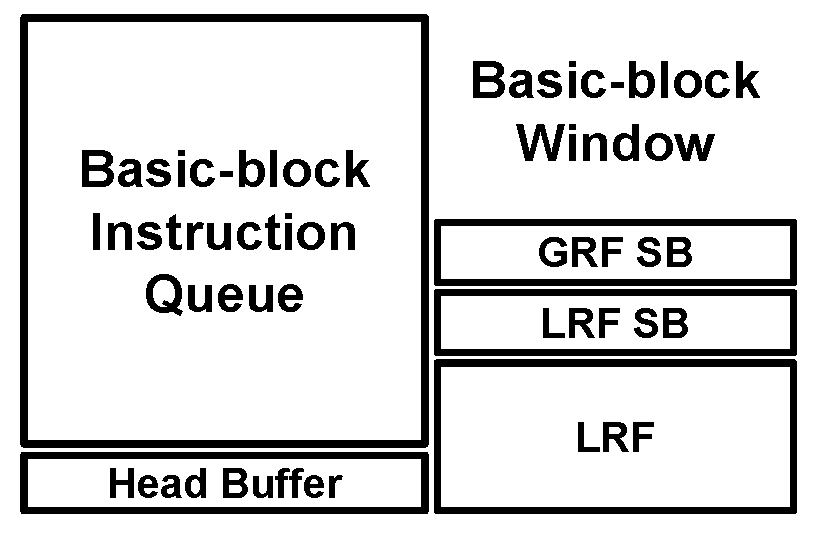
\includegraphics[width=1.0\columnwidth]{fig/bb_window.pdf} 
	\caption{Basicblock window structure}
	\label{fig:bb_window}
\end{figure}

What: discuss bb binary structure including its header contents: branch address.
Also explain the hardware support structure to hold register renamed values for
each global operands (both rad and write). it also contains the BB SN.

Why: to show how we save energy by BP lookup and energy efficient renaming
(renaming buffer is tiny, and cheap to access for both ready-check and wake-up
 logic). energy efficient and more high performance branch prediction.

Header holds: global registers write (for rename), read and offset to the branch
address of the BB.

Branch offset is not kept with BR (so no overhead there)

Instructions hold offset to the instruction rather than to actual register
address. This cuts back the register address by half (making the ISA shorter)
    and also enable RAM lookup to the GRF table upon lookup.

GRF scoreboard update is CAM baesd, but its lookup is RAM based. (very cheap)
    update: CAM lookup to address ready bit
    lookup: RAM lookup to the 1bit entry.

LRF scoreboard udpate and lookup are RAM based. 1bit per entry.


(make a note that bb header for holding register operands is a CAM array)

% Basicblock boundaries are explicitly annotated by the compiler in the program
% binary through special header instructions (H) that contain certain key
% information about the BB; H instructions hold the BB branch instruction address
% (unless the BB is terminated without a branch or jump operation), global read
% registers, and global write registers used in the BB. Figure XX illustrates the
% organization of each H instruction.
% 
% Contrary to existing processors where the branch-prediction unit (BPU) is looked
% up on every fetch group regardless of the type of instructions in the fetch
% group, BB looks up the branch predictor only through H instructions. Immediately
% after the decode stage, H instructions feed the address of the upcoming branch
% instruction to BPU to find the PC of the next basicblock. This approach
% significantly reduces the traffic to BPU reducing mis-predictions due to
% aliasing and lookup energy consumed unnecessarily by non-branch instructions.
% 
% Global write registers used by instructions in the basicblock are incorporated
% in H so that ?.
% 
% Global read registers used by instructions in the basicblock are incorporated
% in H so that the wake-up logic would simply ?.
% 
% Discussion on instruction overhead (for i-cache) of adding H instructions to the ISA.
